% ------------------------------------------------------------------------------
% TYPO3 Version 9.1 - What's New - Chapter "Changes for Integrators" (English Version)
%
% @author	Michael Schams <schams.net>
% @license	Creative Commons BY-NC-SA 3.0
% @link		http://typo3.org/download/release-notes/whats-new/
% @language	English
% ------------------------------------------------------------------------------
% LTXE-CHAPTER-UID:		3a9852ea-e2360d9d-1ff5eec1-a7de3f9f
% LTXE-CHAPTER-NAME:	Changes for Integrators
% ------------------------------------------------------------------------------

\section{Changes for Integrators}
\begin{frame}[fragile]
	\frametitle{Changes for Integrators}

	\begin{center}\huge{Chapter 2:}\end{center}
	\begin{center}\huge{\color{typo3darkgrey}\textbf{Changes for Integrators}}\end{center}

\end{frame}

% ------------------------------------------------------------------------------
% LTXE-SLIDE-START
% LTXE-SLIDE-UID:		31b70474-edcc2a8a-d4a5fd3d-58734dc5
% LTXE-SLIDE-TITLE:		EXT:impexp - Maximum Number Of Records Restriction Removed
% LTXE-SLIDE-REFERENCE:	Deprecation-83592-ImpexpRemovedMaximumNumberOfRecordsRestriction
% ------------------------------------------------------------------------------

\begin{frame}[fragile]
	\frametitle{Changes for Integrators}
	\framesubtitle{Import/Export}

	Various updates have been done to the system extension \texttt{impexp}:

	\begin{itemize}
		\item Restriction "maximum number of records" has been removed\newline
			\smaller
				When exporting pages or records, the restriction to export
				only a maximum number of records has been removed.
			\normalsize

		\item Restriction "maximum file size" has been removed\newline
			\smaller
				When exporting files using the "Export" interface, the
				restriction to only export files of a certain maximum size
				has been removed.
			\normalsize

		\item Size handling removed\newline
			\smaller
				When exporting or importing structures, records and files wrote
				size information to export files and checked these during import.
				This change has no impact on editors.
			\normalsize

	\end{itemize}

\end{frame}

% ------------------------------------------------------------------------------
% LTXE-SLIDE-START
% LTXE-SLIDE-UID:		0504ca33-7c23eff4-93a728fa-bd911c92
% LTXE-SLIDE-TITLE:		Redirect Functionality Moved To Redirects Module
% LTXE-SLIDE-REFERENCE:	83638-RedirectFunctionalityMovedFromSys_domainToRedirectsModule
% ------------------------------------------------------------------------------

\begin{frame}[fragile]
	\frametitle{Changes for Integrators}
	\framesubtitle{Redirect Functionality}

	\begin{itemize}
		\item Option to configure a redirect, when a domain was added to a specific
			page or page branch, has been removed
		\item Setting up redirects can now be done in the new module\newline
			\textbf{Site Management} \textrightarrow \textbf{Redirects}
	\end{itemize}

	\begin{figure}
		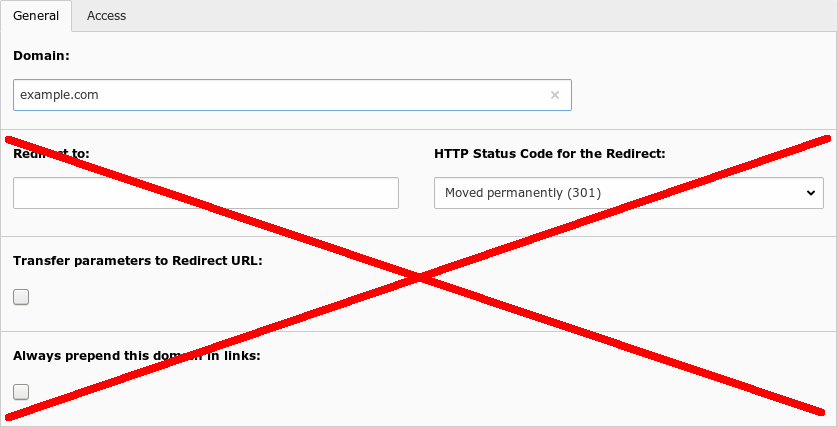
\includegraphics[width=0.6\linewidth]{ChangesForIntegrators/RedirectFunctionalityMovedToRedirectsModule.png}
	\end{figure}

\end{frame}

% ------------------------------------------------------------------------------
